\documentclass[]{llncs}

\usepackage[utf8]{inputenc}
\usepackage{hyperref} 
\usepackage[parfill]{parskip}
\usepackage{graphicx}
%tweak \url{...}
\usepackage{url}
%\urlstyle{same}

%improve wrapping of URLs
\makeatletter
\g@addto@macro{\UrlBreaks}{\UrlOrds}
\renewcommand\subsubsection{\@startsection{subsubsection}{3}{\z@}%
                       {-18\p@ \@plus -4\p@ \@minus -4\p@}%
                       {0.5em \@plus 0.22em \@minus 0.1em}%
                       {\normalfont\normalsize\bfseries\boldmath}}
\makeatother

\setcounter{secnumdepth}{3}% Number up to \subsubsection
\providecommand{\keywords}[1]{\textbf{Keywords: } #1}

\begin{document}

%#====================================Cover Settings=====================================#%
\title{%
Identity Management in Healthcare Using Blockchain Technology}

\author{%
João Santos \and
Pedro Salgueiro \and
Vítor Nogueira}

\institute{%
  Universidade de Évora, Portugal
  \\
  \email{m39519@alunos.uevora.pt}
  \\
  \email{pds@di.uevora.pt}
  \\
  \email{vbn@di.uevora.pt}
 }

{\def\addcontentsline#1#2#3{}\maketitle}


%#====================================Abstract===========================================#%

\begin{abstract}
Blockchain technology allows the creation of systems that introduce a number of
benefits over traditional methods used in today's Healthcare systems.  Costs
and risks associated with these systems can be reduced and information can
become transparent and trustworthy to all participants. In this article the
technological foundations that enable this change are explored and analyzed.
The Hyperledger Fabric Network with true private transactions and advanced
security mechanisms was used to serve as the basis for this system.  An
application was created that uses smart contracts to manipulate the ledger. In
this paper we present this system and its impact in Healthcare.

  \begin{keywords}
      Blockchain, Health, Identity, Big Data
  \end{keywords}
\end{abstract}


%#===================================Introduction========================================#%
\section{Introduction}

Health is becoming more digital thanks to the widespread availability of
computing devices.  More and more medical records are stored on a digital
format.  For storing patient clinical data and their identity in a medical
context, the Electronic Health Record (EHR) was created.
 
While all this information should benefit both patient and health professionals
alike, it is not being handled in an effective manner due to problems caused,
in part, due to the fragmentation of the patients identity that naturally
occurs in today's Health Information Systems.

Health is an important topic, for everyone. Healthcare should strive to provide
the best service it can for everyone and everyone should have access to a
quality service. EHR are being generated at an ever increasing rate but most of
the data is not used in a way that puts the patient's privacy and trust at the
forefront.

The purpose of the work presented in this paper is to create and implement a
Blockchain based system for Identity Management in the Healthcare domain. The
patient will be able to manage his data and control its access. Such a system
would be suited to handle the patient’s identity, for example, in hospitals or
clinics and would be able to solve many problems in how data is traditionally
handled in the Information Systems (IS) available in a regular medical
environment.

Blockchain is known as the technology behind the Bitcoin Cryptocurrency,
altough nowadays it is being used for many more purposes that are explored in
the following sections, and its main design goal is to provide security and
immutability to an agreed upon list of records.

A Blockchain runs on a network of computers and the list of records is
replicated in some manner depending on the Blockchain implementation. The first
Blockchain was conceptualized as the public ledger for the Bitcoin
cryptocurrency in 2008 by Satoshi Nakamoto, a pen name of, a still unknown to
this day, individual or organization of individuals.  The network was
implemented in 2009 and many are now finding it has a much broader potential
across many fields, with some implementations even resembling a programming
platform to execute code in an autonomous manner.  \cite{Nakamoto2008}

A single universal way to identify a person in a given environment is clearly
something we should strive towards as seen in, for example, the \textit{Cartão
do Cidadão}, a portuguese identification document that replaces four other
identification documents, streamlining portuguese civilian identification.
This also allows many businesses to tailor their services to this document
making it easier on both parts and eliminating unnecessary costs and risks.

Electronic Health Records (EHR) have seen some progress made regarding the
standards that allow for interoperability between different organizations
thanks to the Health Level 7 (HL7) standard.  While this standard is growing in
use and is represented internationally, Portugal has just started the work
required to implement it.  \cite{HealthLevel7}

In an effort to make the identity of a patient more secure and transparent a
Blockchain can be used to create a system that puts at the forefront of its
design the patients, breaking conventions in traditional patient data handling.

In this article different Blockchain implementations are explored and related
work in this field is presented.  More precisely, in Section~\ref{background},
a brief introduction to Blockchain is made followed by an introduction to its
most prominent implementations. Then a number of real-world use cases of this
technology in the healthcare field are explored. In Section~\ref{HLFHealthcare}
technical details of the system will be presented.  Finally, in
Section~\ref{conclusion},  some conclusions are observed regarding the change
enabled by these advances.


%#====================================Background========================================#%

\section{Background} \label{background}

While Blockchain is not a new concept at this point, it is an evolving
technology that is being used to solve old problems with new approaches. This
section will explore the Blockchain technology origins and history, some of its
different implementations and a brief history to the identity problem is
presented.

\subsection{Blockchain Technology}

A Blockchain can be many things. It can refer to the Bitcoin Blockchain,
alternative implementations or forks of the Bitcoin Blockchain called Altchains
or even platforms that allow execution of code in an autonomous manner, exactly
as it was programmed, with no human intervention.  It is a continuously growing
list of records, written in the ledger, a structure where records are written,
that is being replicated across a network of devices in opposition to having a
single central record history, making it a good example of a distributed
database.  \cite{Wood2017}
  
The main design goal of the Blockchain is security and to fulfill this purpose
it uses techniques such as cryptography and digital signatures to not only
verify the authenticity of records but also read or write access to the
network.

Unlike a conventional central data storage, where only a single entity keeps a
copy of the underlying database, the ledger of the Blockchain is replicated
across any number of nodes.  Not every participant has the same ability to
interact with the ledger and in this respect a Blockchain can be permissionless
or permissioned. In a permissionless Blockchain every node of the network can
write in the Blockchain whereas in a permissioned Blockchain only a select
group of entities have access to writing in the ledger, making the permissioned
version, by default, secure if the entities themselves are secure and
considered trustworthy.

How does a permissionless Blockchain maintain security if every participant has
access to writing on it, including potentially malicious parties?

Take for example the Bitcoin Blockchain that uses a peer-to-peer network to
avoid meddling from a financial institution or a third party in a financial
transaction. Given that participating nodes in the network can belong to
different and often competing parties, there is no implied trust between them,
so the Blockchain needs a mechanism to ensure the integrity of the ledger and
prevent malicious meddling from interested parties or to avoid a central
authority.\cite{Barclay2017}

To solve this problem, consensus mechanisms are used differently, depending on
its implementation, but having, at its core, a solution to create immutable
records and ensure security.  In Bitcoin Blockchain’s case, consensus is
reached by the longest chain rule where the longest chain not only serves as
proof of the sequence of events witnessed, but as proof that it came from the
largest pool of computing power.\cite{Baars2016}

While the first Blockchain was conceptualized as the public ledger for the
Bitcoin cryptocurrency in 2008 by Satoshi Nakamoto and implemented in 2009,
many are now using it as a foundation across many application areas such as
identity management, traceability and asset management.  Thanks to the roaring
success of Bitcoin and the increasingly apparent use cases that the Blockchain
can provide, the public awareness of it is rising and it is quickly becoming a
technological foundation in our economic and social systems.
% Need References for this

\subsubsection{Ethereum}

Bitcoin is getting media coverage almost everyday and public awareness in
cryptocurrencies in general is rising.  Some people are considering
cryptocurrencies and the Blockchain, to be essentially the same technology and,
while that may have been somewhat true not so long ago, Blockchain technology
is starting to be used in a plethora of ways.

Ethereum is an open-source platform based on the Blockchain technology that
enables developers to build and deploy Decentralized Applications
(\textit{DAPPs}).  Ethereum is being developed by the Ethereum Foundation and
was first discussed by Buterin in 2013.  Ethereum intends to provide a
Blockchain with a built-in programming language that is used to create
\textit{Smart contracts}.  \cite{Wood2017}

These contracts are used to describe the logic of any system that developers
can imagine and, when created, can then be deployed to the Blockchain where
they execute as “autonomous agents”.  Thanks to these tools it is safe to say
that long gone are the days where building Blockchain applications required a
complex background in coding cryptography, mathematics as well as significant
resources.\cite{Wood2017,BlockGeeks2017}

Ethereum Blockchain is a permissionless Blockchain, and thus, it must have a
consensus mechanism to ensure the validation process of every record and, in
turn, ensure security and immutability. While other implementations of the
Blockchain have different consensus mechanics, in Ethereum’s case, all
participants have to reach consensus over the order of all transactions that
have taken place. If a definitive order cannot be established then a
double-spend might have occurred.

\subsubsection{Fabric}

Hyperledger Fabric (HLF) is part of the
\href{http://www.hyperledger.org/projects/fabric}{Hyperledger} project started
in December 2015 by the Linux Foundation, and is an open-source
developer-focused community of communities focused on the development of
enterprise-grade, open-source Blockchain-based solutions.  Fabric is an
implementation of a Distributed Ledger Platform (DLP) under the Hyperledger
umbrella.  \cite{Cachin2016}

HLF’s initial commit was contributed by IBM and written in Go language.  It is
a permissioned Blockchain and its main design goal was to surpass previous
Blockchain implementation limitations, such as, lack of true private
transactions and confidential contracts.

This is achieved thanks to assigning peers in the network three distinct roles
and by offering the ability to create channels each with its own private
ledger.  A peer can have the role of endorser, committer or consenter or
sometimes multiple roles.  HLF is intended as a foundation for developing
applications in a modular fashion, opting for a plug-and-play approach to
various components. \cite{HyperledgerFabricDocs2017}

HLF, as discussed, also allows the creation of smart contracts which can be
written in Chaincode.  As this Blockchain's key operational requirement is
privacy, true private transactions and confidential contracts can exist and are
a great asset for a business environment where sensitive information is
necessary and disclosed often.  Thanks to its modular approach consensus
protocols are no longer hard-coded and trust models can be repurposed.

\subsubsection{Burrow}

Hyperledger Burrow (HLB) is also part of the Hyperledger project and its
development started in 2014 by Monax and sponsored by Intel. It is a
permissionable smart contract machine written in Go and offers a modular
Blockchain client with a permissioned smart contract interpreter built, in
part, to the specification of the Ethereum Virtual Machine (EVM) and the client
has, essentially, three main components, the consensus engine, the permissioned
EVM and the Remote Procedure Call (RPC) gateway.
\cite{Kuhlman2017,HyperledgerBurrow2017}

HLB has its own Consensus Engine, the Byzantine fault-tolerant Tendermint
protocol.  The Tendermint protocol is an open-source effort that allows high
performance in solving the consensus problem and also has a flexible interface
for building arbitrary applications above the consensus, as well as, a suite of
tools for deployments and their management. \cite{Buchman2016}
%
%#===========================Identity in
%Healthcare===================================#%

\subsection{Identity in Healthcare} Originally records of a patient were stored
in a physical format.  Thanks to the advent of the computers more and more
records are stored on a digital format and the Electronic Health Record (EHR)
was created.  This benefits handling of information between the patient and the
medical professionals and medical institutions. But first we must discuss what
is defined as identity in this specific case.

Identity is a construct that depends on the context.  Identity can be defined
as the characteristics determining who or what a person is.  In this paper we
define identity as the set of characteristics that determine who is the patient
in the given Healthcare ecosystem they belong to, such as, the name, the age,
the cellphone number, the gender and the birth date of the patient.  Electronic
Health Records encapsulate this information in digital format, however, they
are usually represented in a format according to the Information System they
were designed to work with.

To enable interoperability, standards for EHRs were created and many failed to
bring the much needed consensus that was required for interoperability between
different Information Systems in different institutions.  Health Level 7 has
done much work to be recognized in many countries and is quickly being
implemented in many countries to allow for joint efforts between organizations.

Even with these advances in mind, the nature of many clinics and hospitals
Information Systems makes the management of their patients identity a very
cumbersome, costly and risky affair to handle.  Security in a connected age,
where internet is easily available, is lagging behind and presenting some
problems.  There is also the question of transparent use of information by the
organizations that store it.
%
%#===========================Related Work===================================#%

\subsection{Blockchain for Identity Management in Healthcare: Use Cases} Some
companies have already started developing Blockchain applications in the
Healthcare field and established some key partnerships.

Many Blockchain-based solutions are still very early on development or
deployment.  One exception is Guardtime, that has fully deployed their system
in 2008, started cooperating in 2011 and in 2016 announced a partnership with
the Estonian Government, where a million patient records are now secured by the
strategy and, until today, still proves the resilience of the Blockchain
technology, as well as, other advances in cryptography.  Now other companies
like Verizon are becoming interested in this technology for their own purposes.
\cite{GuardTime2018,EstonianGovernmentGuardTime2016}

Another company, Gem, is collaborating with Phillips Healthcare to explore
options in this area, and is opting to solve the interoperability problem with
an additional layer of abstraction they call GemOS.  Factom, another
Blockchain-based service, has also announced a partnership with a major US
medical services provider
HealthNautica.\cite{BlockchainCompHealth2017,FactomPartnership2017}

The use of the Blockchain technology in the health field is expanding. Just
recently a new platform appeared, called Medichain that allows patients to
store their own data in a secure way and give anonymized access to this data to
specialists. Giving data allows for users to gain tokens that represent value.
\cite{MediChain2018}

%#==============Patient Identity Representation in Blockchain==========================#%

\section{A HLF Network for Healthcare} \label{HLFHealthcare} Altough many use
cases were presented in Section~\ref{background} they do not have the
technology that allows true private contracts and some of them use a currency
as a means to ensure the network consensus is achieved, by monetizing the
patients data.  After analyzing the different Blockchain implementations the
Fabric network was chosen as the foundation for this system. This
implementation was chosen to overcome previous works weaknesses and to match
the security and privacy that patients expect to have with their health data.
First we will discuss the tools provided to configure the network, and then
discuss the system architecture.

\subsection{Fabric Network Configuration Tools}

Hyperledger Fabric (HLF) does not use a centralized ledger where every record
is available to every participant in the network.  Instead it opts to allow
multiple ledgers in a network to achieve different goals of a greater purpose.
This allows the creation of channels of information between trusted parties,
for example, a channel of secure and private information between the clinical
staff of an hospital and a patient.

A HLF network is comprised by the \textit{cryptogen}, \textit{configtxgen},
\textit{configtxlator} and \textit{peer} tools that are used to configure the
network.

The \textit{cryptogen} tool generates cryptographic data consuming the file
\textit{crypto-config.yaml}.  HLF uses an abstraction layer for certification
and authority called Membership Service Provider (MSP) that defines the rules
by which entities are governed and authenticated and it must be unique for
every participating entity.

The \textit{configtxgen} tool generates the genesis block for the orderer
services and the initial transactions.  This tool consumes the file
\textit{configtx.yaml} that defines configuration parameters for channels, the
genesis block and the orderer service.

The \textit{configtxlator} tool is also used to generate channel configurations. 
Finally the \textit{peer} tool is used to manage the participating peers in the HLF network.

These tools are used to create and maintain the topology of the network and are
invoked when a change to the network is made, for example, when permissions to
certain records are changed or a new user is enrolled in the network and are
very much intertwined with the Certificate Authority (CA) server system to
maintain the security that is needed in a sensitive subject that deals with
private information.

\subsection{Identity Representation in Hyperledger}
 
HLF allows information to be written and read in a distributed manner with
security and privacy at the forefront. Using smart contracts, a record is
created to represent the concept of identity in this network.

The information that defines the patients identity is a key requirement to
build a system that recognizes patients across the Healthcare environment, as
discussed in Section~\ref{background}.  To this end, the identity of a patient
is recorded on the ledger of the HLF network as a structure via a smart
contract deployed to the network that interacts directly with the ledger.  This
structure contains the necessary fields to identify the patient such as its
name and birth date, for example, as well as some other information necessary
to manage this data. 

To aid in interoperability with other systems, as seen in Figure
\ref{fig:interoperability}, the Fast Healthcare Interoperability Resources
(FHIR) standard by the Health Level 7 organization was used as basis for the
representation of a patient.  Each field of the structure that represents the
patients identity, defined in the smart contract, is linked to a field of the
\href{http://www.hl7.org/fhir/patient.html}{patient structure as presented in
the FHIR standard}.

\begin{figure}[ht]
\centering
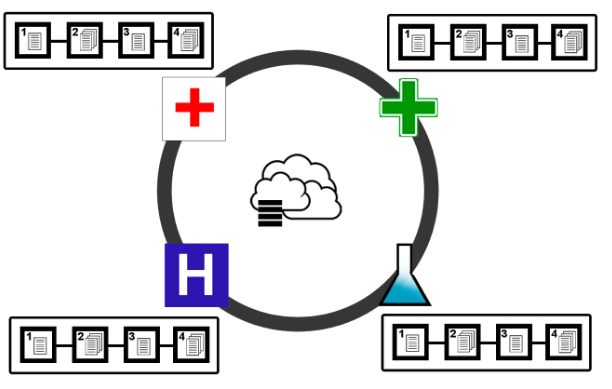
\includegraphics[width=0.7\linewidth]{images/interoperability.png}
\caption{\label{fig:interoperability}An Example of Interoperability with the Blockchain Network}
\end{figure}

\subsection{Application and Smart Contracts}

To create an interactive system that can manage the patients identity in an
Healthcare environment an application was built that the user interacts with.
This application interfaces with smart contracts through the Hyperledger Fabric
Software Development Kit and the chaincode was built using the Hyperledger
Fabric Shim for node.js.

The application is accessed by the user and calls upon the smart contract.  The
smart contract will handle the assets part of the system.  A smart contract to
represent and manipulate identity was built and interfaces with the network to
write and read records to the appropriate ledger. The overview of the
architecture for this system is represented on Figure \ref{fig:appOverview}.

\begin{figure}[ht]
\centering
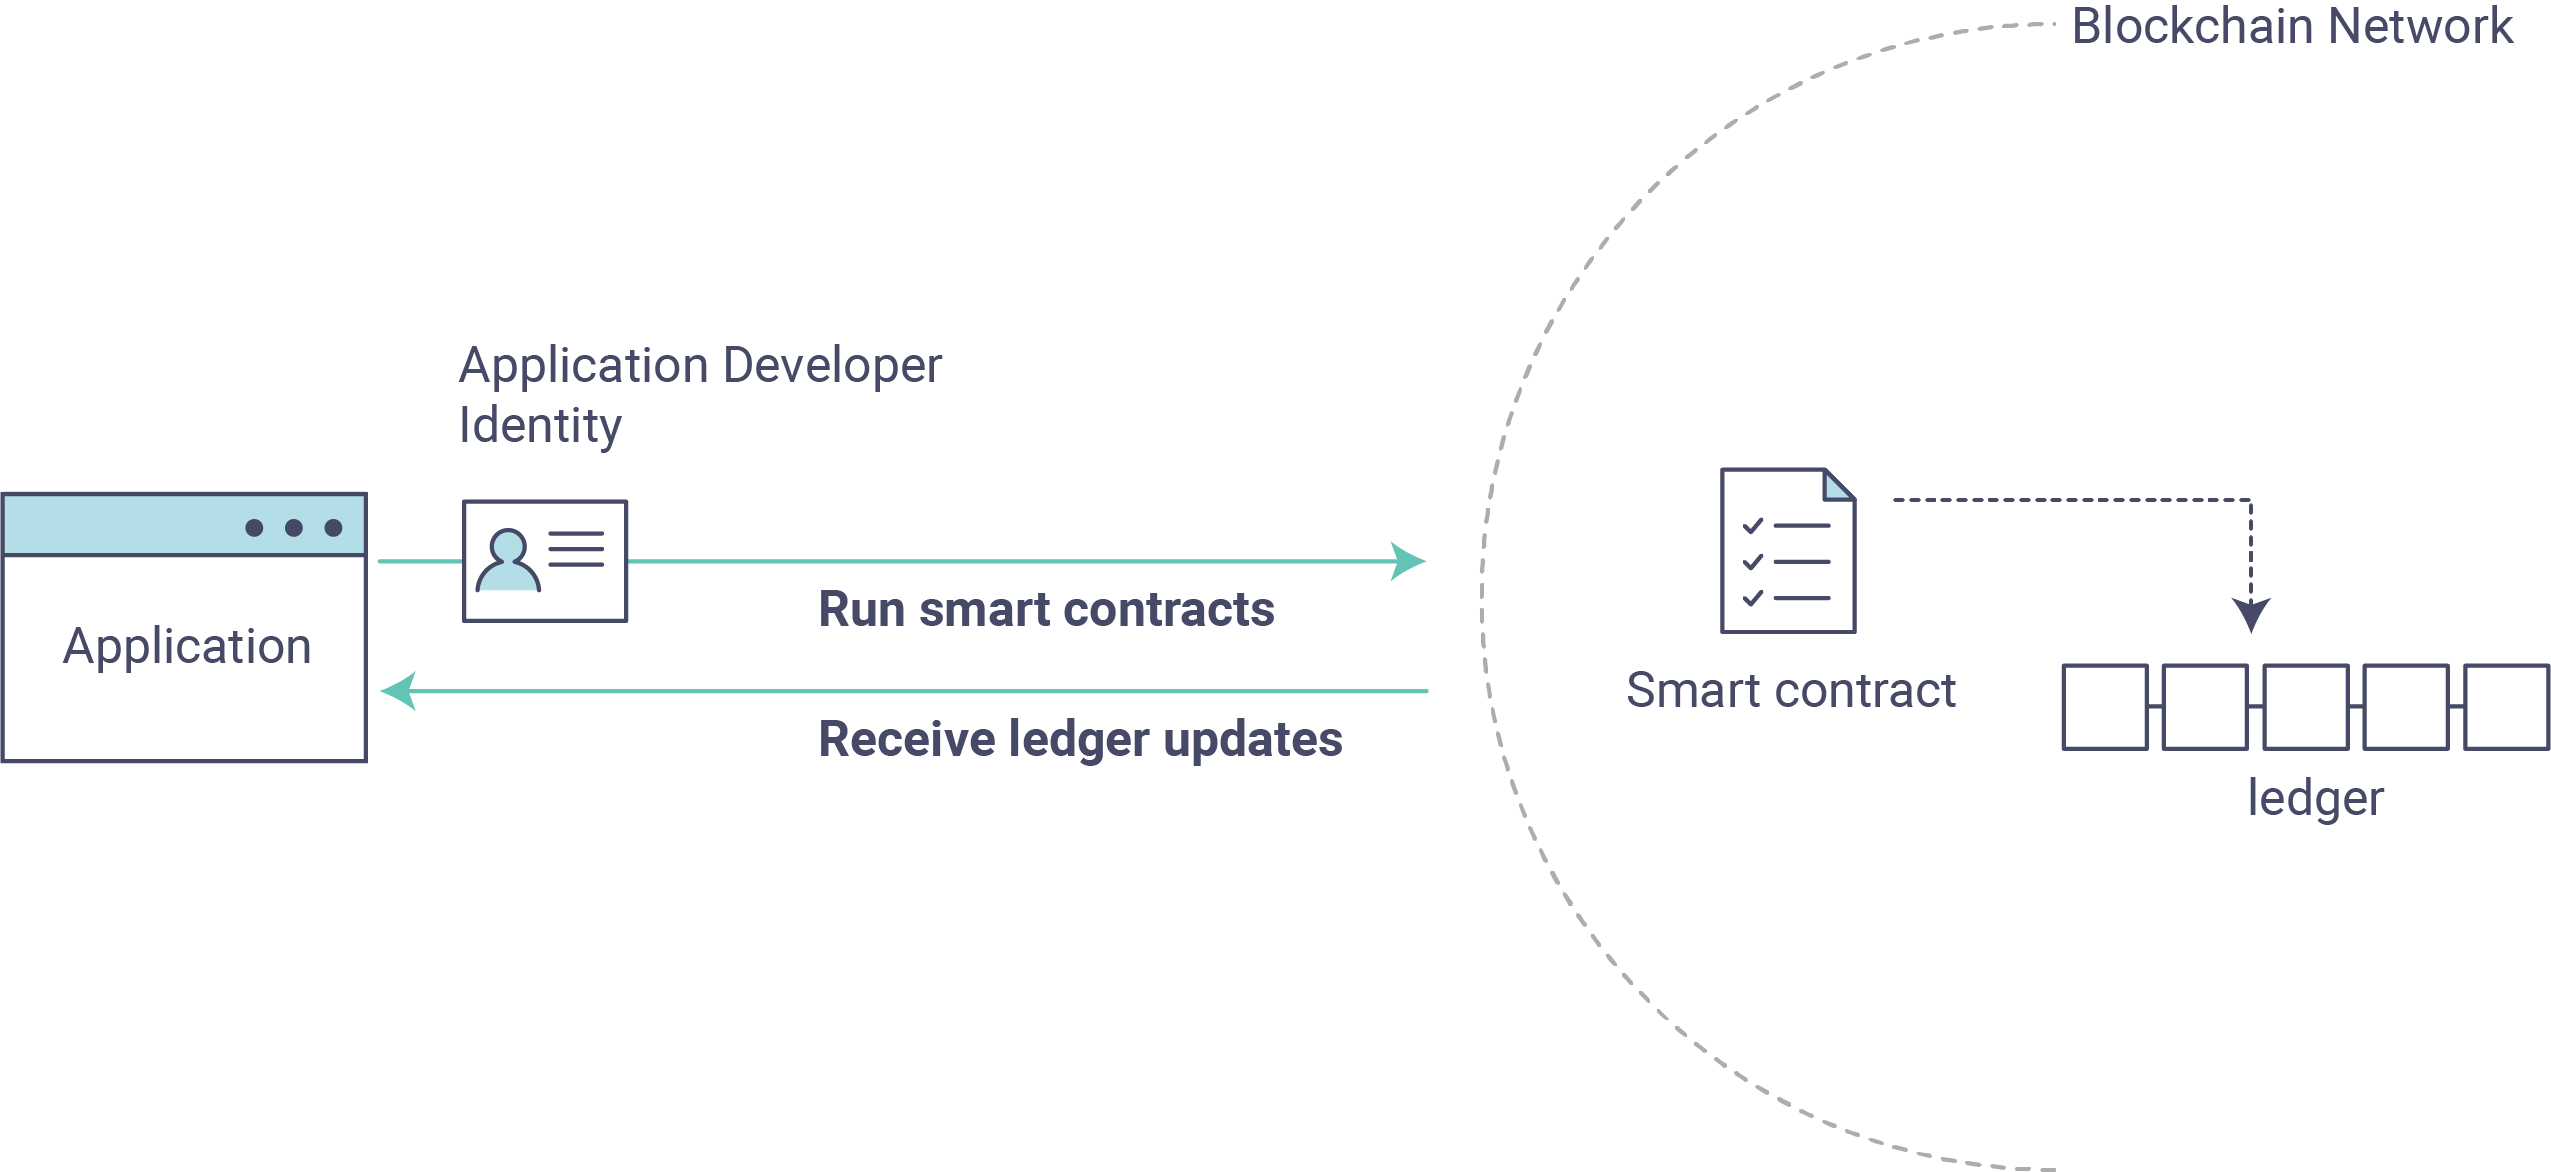
\includegraphics[width=1\linewidth]{images/hyperledgerAppOverview.png}
\caption{\label{fig:appOverview}An Overview of the System Architecture (Source: \href{http://hyperledger-fabric.readthedocs.io/en/latest/write_first_app.html}{HLF Fabric Documentation})}
\end{figure}

The application allows for user enrollment to create a new identity in the
network.  When a new user of the application enters the network; the function,
in the smart contract, that initializes the creation of the user and writes the
user to the ledger as a new participating identity is called. Due to the
security mechanisms this specific transaction is automatically signed by the
administrator of the network and is verified by the CA servers.

The smart contract also provides the application with several operations to
manage the identity object as seen on Figure \ref{fig:smartContractOverview}.
These operations form an Application Programming Interface (API) that return a
payload in JSON format with identity information from the network.  This API
allows a query to be made to the network that returns the patients information,
changing incorrect or outdated information or disabling the identity structure
of someone who is not participating in the network actively anymore in order
for that information to be read-only from that point on, for example, with more
available.  Depending on the operation only certain users can access the
information or manipulate the already existing one.  This system architecture
leads to a modular as well as extensible approach regarding the availability of
new operations that become available as soon as new versions of the smart
contract are deployed.  \begin{figure}[ht] \centering
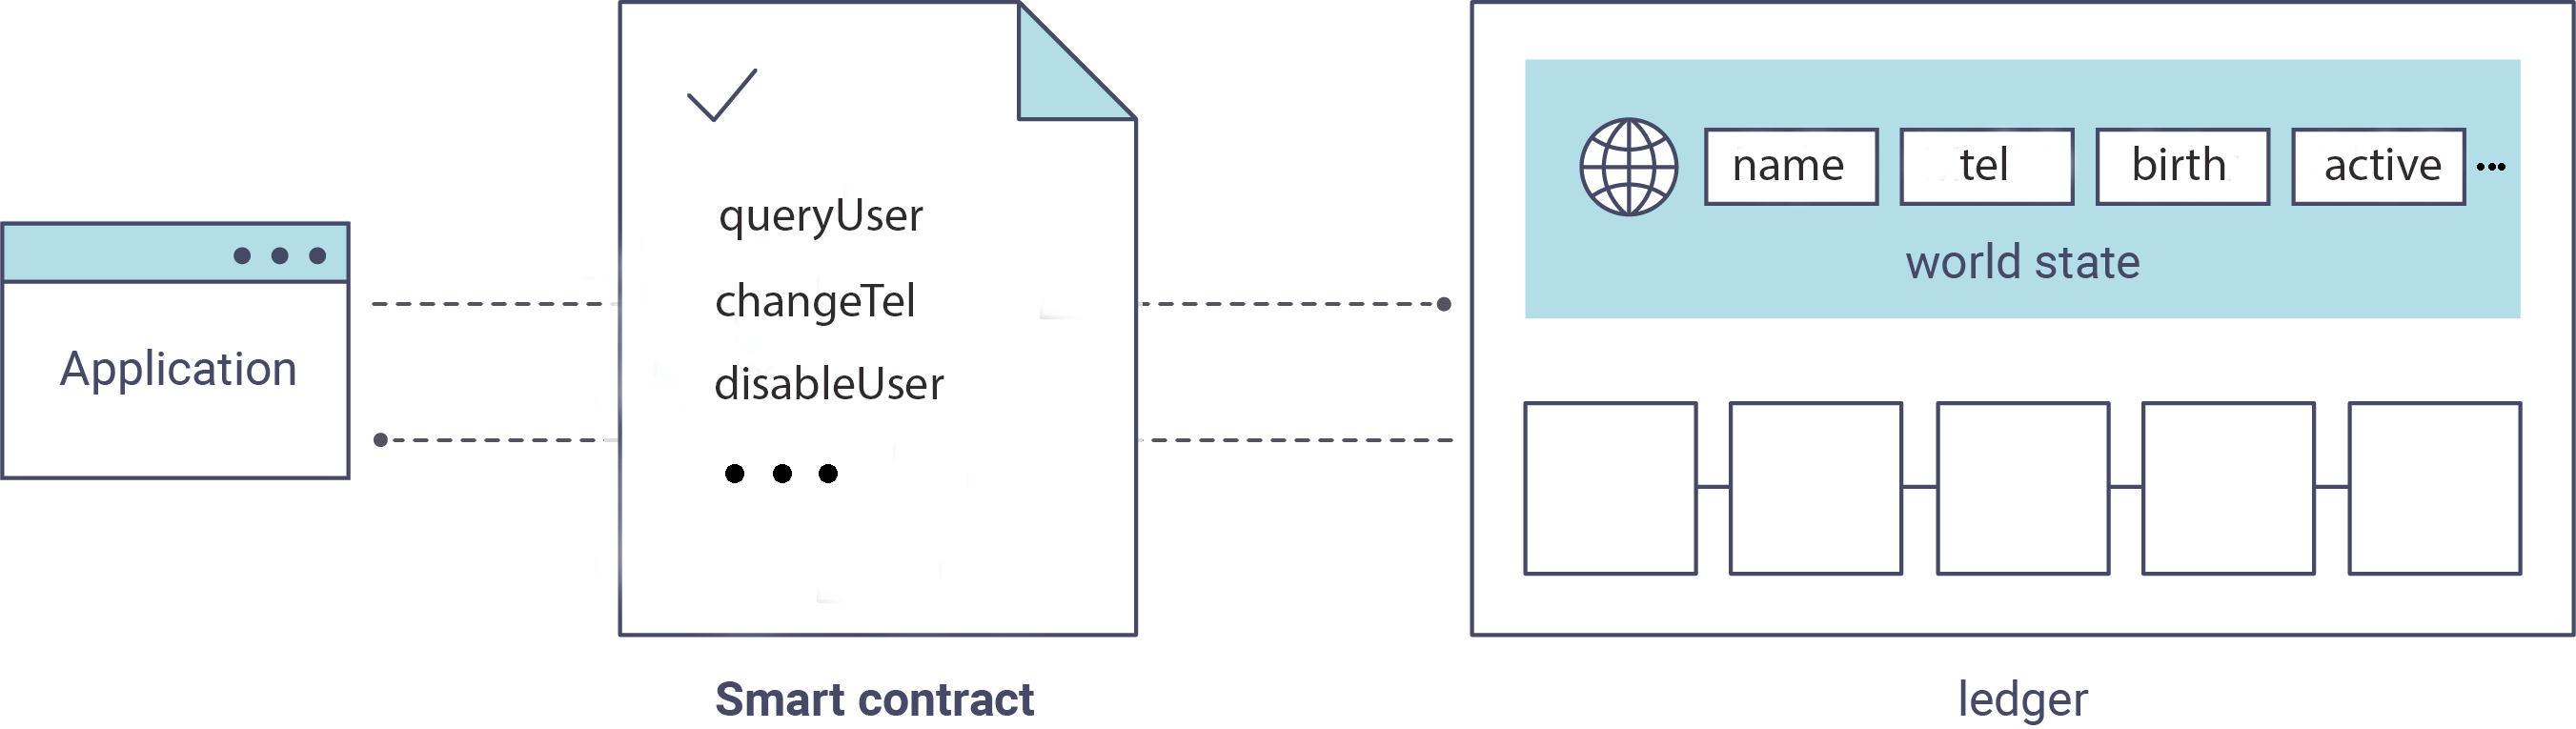
\includegraphics[width=1\linewidth]{images/smartContractOverview.png}
\caption{\label{fig:smartContractOverview}Smart Contract Operations Example
(Original:
\href{http://hyperledger-fabric.readthedocs.io/en/latest/write_first_app.html}{HLF
Fabric Documentation})} \end{figure} \newpage
%#===========================Conclusion===================================#%

\section{Conclusion} \label{conclusion} In this document it was described that
the way identity is handled by medical institutions nowadays presents a
problem. Blockchain was explored as a tool to solve this problem and some of
its different implementations were analyzed. Some practical use cases of this
technology were also discussed.  This research will enable solid foundations
for future work.

It is safe to say that a system for improving the way a patient can interact
with their health data can be built, using this technology, as discussed in
previous sections.  The system should allow for a transparent handling of
personal data and be able to allow for secure management of access to this
particular data.

If an advance is made in this regard it is expected that the patients trust in
their Healthcare service is increased, and that risks and costs inherent to
multiple independent information systems, that are not normalized to any
standard, be reduced. 
%#====================================Bibliography========================================#%


\begingroup
\nocite{*}
\raggedright
\bibliographystyle{alpha}
\bibliography{bibliography}
\endgroup

\end{document}
